%! Tex program = pdflatex
\documentclass[UTF8]{ctexart}
\CTEXsetup[format={\Large\bfseries}]{section}
\usepackage{amsmath}
\usepackage{ctex}
\usepackage{array}
\usepackage{ulem}
\usepackage{graphicx}
\usepackage{geometry}
\usepackage{multirow}
\usepackage{subfigure}
\usepackage{float}
\usepackage{multicol}
\usepackage{multirow}
\usepackage{indentfirst}
\usepackage{stfloats}
\usepackage{makecell}
\geometry{papersize={21cm,29.7cm}}
\geometry{left=2.54cm,right=2.54cm,top=3.18cm,bottom=3.18cm}
\usepackage{fancyhdr}
\pagestyle{fancy}
\lhead{\today}
\chead{}
\rhead{2020011075}
\lfoot{清华大学}
\cfoot{\thepage}
\rfoot{物理实验B(1)}
\renewcommand{\headrulewidth}{0.4pt}
\renewcommand{\headwidth}{\textwidth}
\renewcommand{\footrulewidth}{0pt}
\usepackage{bm}
\begin{document}
\begin{titlepage}
    \begin{center}
		\quad \\
		\quad \\
        \quad \\
        \quad \\
        \quad \\
        \quad \\
		\kaishu \fontsize{30}{15} 分光计的调节和色散曲线的测定

	\end{center}
	\vskip 10cm

    \begin{center}
        \begin{large}
        \begin{tabular}{cc}
        院系班级:& ~~~~~~自动化系~自02班~~~~~~    \\
        \cline{2-2}\\
        学生姓名:& 彭程    \\
        \cline{2-2}\\
        学\qquad 号:&2020011075   \\
        \cline{2-2}\\
        组\qquad 号:& 单一晚M    \\
        \cline{2-2}\\
        座~~位~~号:& \# 13    \\
        \cline{2-2}\\
        实验时间:&2021.11.8\\
        \cline{2-2}\\
        指导老师:&孙家林\\
        \cline{2-2}
        \end{tabular}
        \end{large}
        \end{center}

\end{titlepage}
\newpage
\tableofcontents
\newpage
\section{实验目的}
\begin{enumerate}
\item 了解分光计的原理与构造,学会调节分光计;

\item 用最小偏向角法测定玻璃折射率;

\item 掌握三棱镜顶角的测量方法(自准法)。
\end{enumerate}


\section{实验仪器}

\noindent 实验仪器有:分光计,平面反射镜,玻璃三棱镜,氦光谱管及其电源。

\noindent 其中, 氦光谱管是将稀薄的氦气封闭在玻璃管内制成。管的两端各装一个电极(勿用手触碰电极),两电极
间加高电压后产生放电并且发光,通过三棱镜分光可得到氦的线状光谱。

\section{实验原理}
\subsection{分光计的结构及调节}

\noindent  \textbf{1、 简述分光计的主要结构和部件包括哪些}

主要结构包括平行光管、望远镜、度盘和平台。


\noindent  \textbf{2、 简述要用分光计测准入射光与出射光之间的偏转角必须满足的两个条件是什么?}

(1)入射光和出射光均为平行光;

(2)入射光和出射光的方向以及反射面或折射面的法线与分光计的刻度盘平行。

\noindent  \textbf{3、 简述分光计调整的目标是什么?}

(1)平行光管发出平行光

(2)望远镜适合接受平行光

(3)平行光管光轴、望远镜光轴、以及平台上光学元件的法线与主轴垂直



\subsection{用自准法测三棱镜顶角A的测量原理}

    \begin{figure}[H]
        \centering
        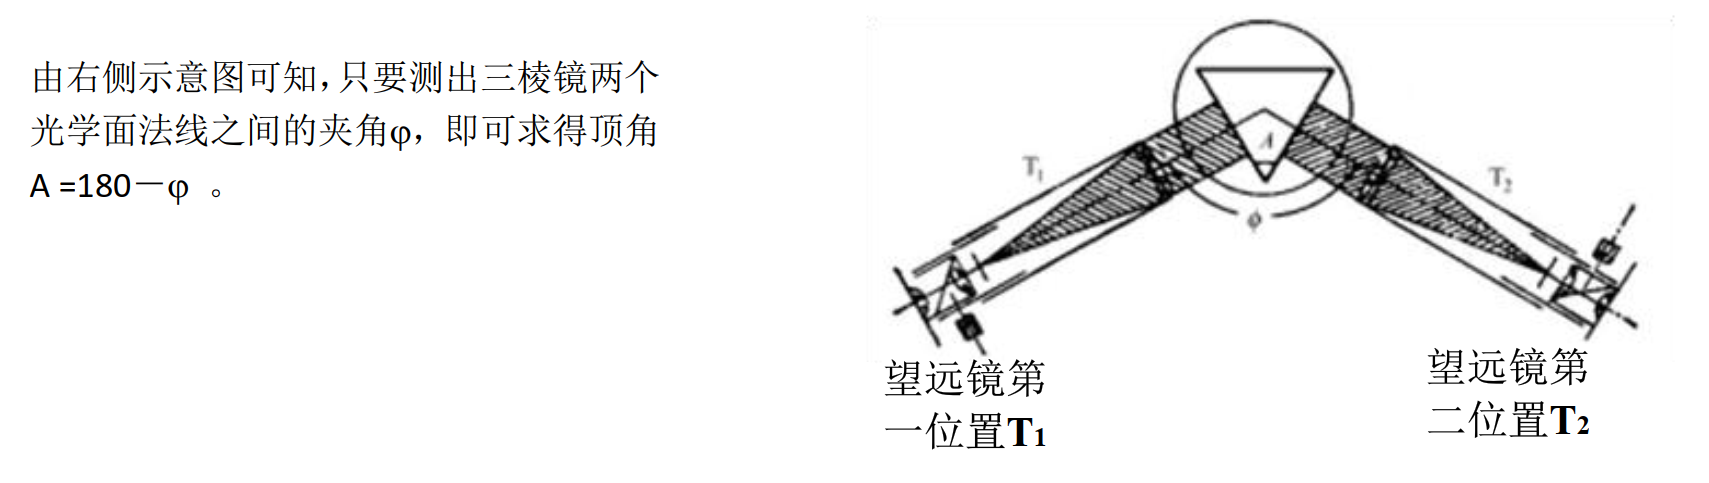
\includegraphics[scale=0.55]{自准法原理.png}
    \end{figure}

\subsection{用最小偏向角法测玻璃折射率的原理}

    \begin{figure}[H]
        \centering
        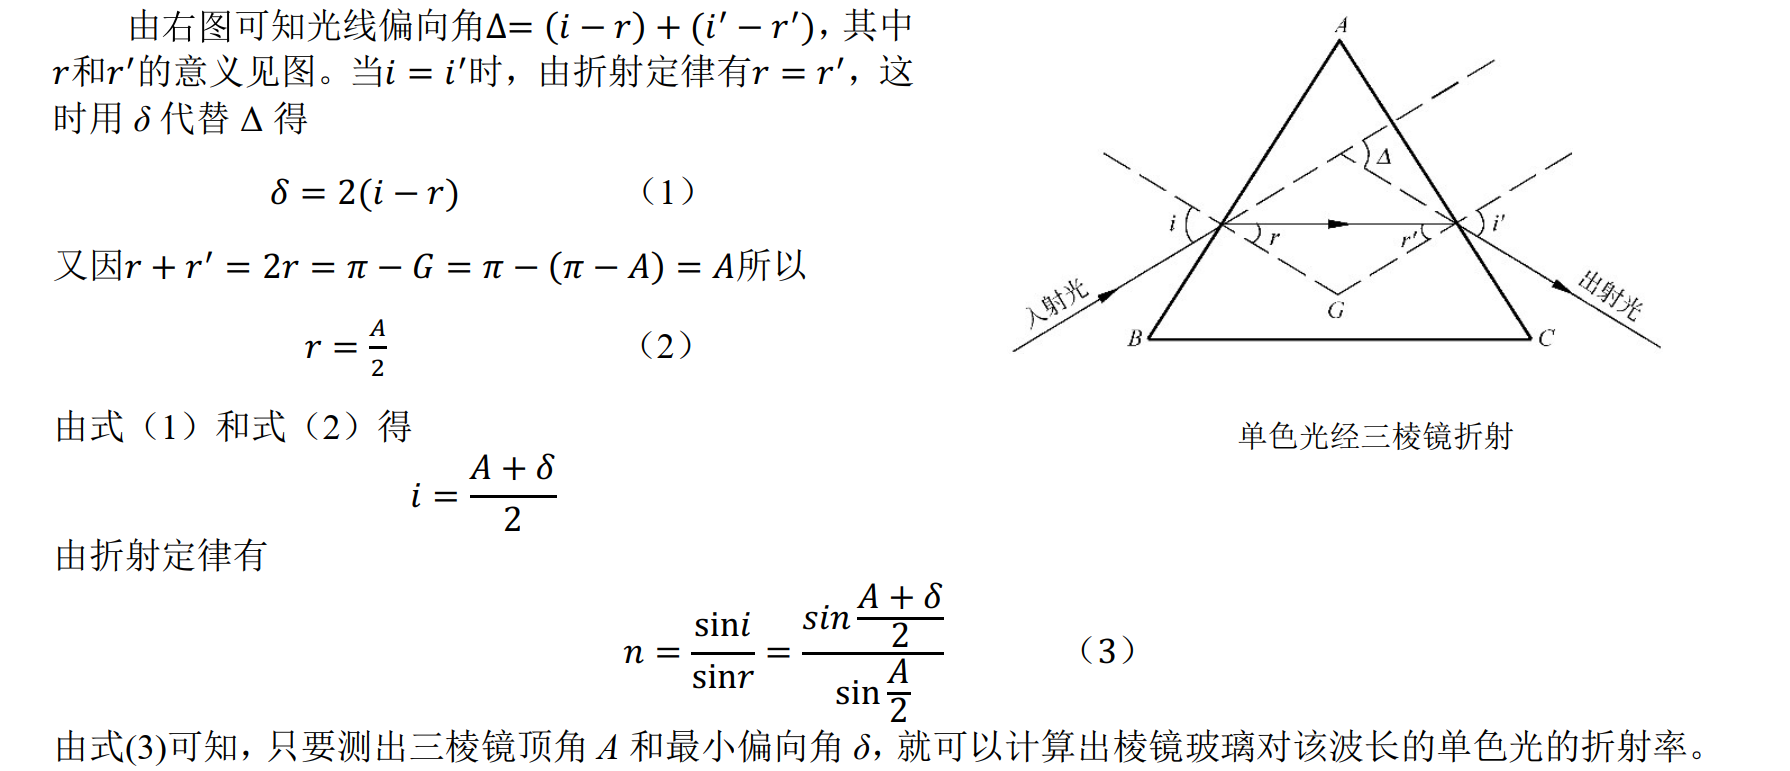
\includegraphics[scale=0.55]{最小偏向角原理.png}
    \end{figure}
    

\section{实验步骤}

\noindent  \textbf{一、 调节望远镜适合于观察平行光(简述调节过程及所观察到的现象)}

首先目测粗调使得望远镜与刻度盘大致平行;

之后调节目镜与叉丝的距离,使得视野中的叉丝清晰;

将平面镜放在平台上,转动平台,从望远镜中找到十字形反射像;

调节叉丝套筒,从目镜中看到比较清晰的十字形反射像,将平面反观镜贴于望远镜目镜处,
当调整眼睛的观测角度时十字反射像不在叉丝左右晃动则说明十字形反射像已经和叉丝无视差。
\\

\noindent  \textbf{二、 调节望远镜光轴垂直于分光计主轴(简述调节过程及所观察到的现象)}

将平面反光镜放在平台上,先从反光镜一面找到十字形反射像,旋转$180^\circ$ 后从反光镜另一面找到十字形反射像。
之后利用二分渐进法调整(先调小平台下的俯仰螺钉使十字形反射像与叉丝上交点之间的上下距离减小一半,再调节望远镜的
调水平螺钉使像叉丝上交点重合,然后转动平台 180°进行同样调节,反复几次操作)。

当十字形反射像和叉丝上交点重合,并且当平台旋转180度后,仍然完全重合,则说明望远镜光轴已经垂直于分光计主轴。
\\

\noindent  \textbf{三、 调节平行光管使之产生平行光(简述调节过程及所观察到的现象)}

调节窄缝的宽度以及窄缝与透镜的距离,当从望远镜的目镜中观察到清晰的狭缝像,且狭缝像和叉丝无视差时,
则说明平行光管已产生平行光。
\\

\noindent  \textbf{四、 调节平行光管光轴垂直于分光计主轴(简述调节过程及所观察到的现象)}

调节平行光管的调水平螺钉,当望远镜目镜中观察到的狭缝像中点和叉丝中心交点重合时,说明平行光管光轴垂直于分光计主轴。

实际实验时发现调节过程中十字光源可能遮挡视野,因此不需将狭缝像和叉丝中心线重合,只要两者中心位于同一水平高度即可。
\\

\noindent  \textbf{五、调节三棱镜两个光学面的法线垂直于分光计主轴(简述调节过程及所观察到的现象),测量三棱镜顶角A}

将三棱镜按照两个光学面法线各垂直于平台底部三颗螺丝构成的正三角形的一条边的原则放置
(其目的是调节一颗螺丝时只改变一条法线的方向,而不影响另一条法线与轴线的垂直关系)。
对于每个光学面,调节该面法线对应的那颗螺丝,使得这一光学面产生的十字形反射像与叉丝上交点重合。
当两个光学面的十字形反射像均与叉丝上交点重合时,说明两个光学面法线已经垂直于主轴。

分别记录两个光学面的十字形反射像与叉丝上交点重合时望远镜的位置,两者作差得到$\Phi$,顶角$A=180^\circ-\Phi$。
\\

\noindent  \textbf{六、 调节并确定某谱线的最小偏向角(简述调节过程及所观察到的现象),测量入射光方位和出射
光方位}

先观测入射光的方位:移动望远镜,当狭缝像与叉丝中心线重合时记录入射光方位。

之后观察谱线:在望远镜目镜中找到谱线,将平台稍稍转动,当棱镜转到某个位置时,谱线不再移动,
继续使棱镜沿原方向转动时,谱线反而向相反方向移动,即偏向角反而变大,这个转折位置就是最小偏向角位置。
此时将望远镜叉丝竖线对准此条谱线中心,测量读数减去入射光方位即得到最小偏向角。


\section{数据处理}
\subsection{自准法测量三棱镜顶角数据}

数据记录如下:

\begin{center}
    \begin{tabular}{|c|c|c|}
        \hline &  ~~~~~~~~游标 I~~~~~~~~&  ~~~~~~~~游标 II~~~~~~~~ \\
        \hline  第一位置 $ T_{1}$ & $155^{\circ} 44^{\prime}$ & $335^{\circ} 47^{\prime}$ \\
        \hline  第二位置  $T_{2}$ & $35^{\circ} 46^{\prime} $& $215^{\circ} 43^{\prime}$ \\
        \hline $\phi_{i}=\left|T_{1}-T_{2}\right|$ & $119^{\circ} 58^{\prime}$ & $120^{\circ} 4^{\prime}$ \\
        \hline $\Phi=\frac{1}{2}(\Phi_1 -\Phi_2)$&\multicolumn{2}{c|}{$120^{\circ} 1^{\prime} $}\\
        \hline
    \end{tabular}    
\end{center}

根据数据计算得:
$$
A=180^{\circ}-\Phi=59^{\circ} 59^{\prime}  
$$

不确定度:
$$
\Delta_{A}=\sqrt{2}^{\prime} \approx 1.4^{\prime}
$$

则  A  的测量结果为  
$$
A=59^{\circ} 59.0^{\prime} \pm 1.4^{\prime} 
$$

\subsection{测量三棱镜最小偏向角数据}


入射光方位的两个游标值分别为:


$\phi_{10}={97}^{\circ} 3^{\prime}, \phi_{20}={277}^{\circ} 4^{\prime}$

\begin{center}
    \begin{tabular}{|c|c|c|c|c|c|}
        \hline 谱线波长  $\lambda / n m$  & 读数  $\phi_{1}$  & 读数  $\phi_{2}$  & $ \delta_{1}=\phi_{1}-\phi_{10}$  &  $\delta_{2}=\phi_{2}-\phi_{20} $ &  $\delta=\frac{1}{2}\left(\delta_{1}+\delta_{2}\right) $ \\
        \hline  447.1  &  $150^{\circ} 16^{\prime}$  &  $330^{\circ} 19^{\prime}$  &  $53^{\circ} 13^{\prime}$  &  $53^{\circ} 15^{\prime}$  &  $53^{\circ} 13^{\prime}$  \\
        \hline  471.3  & $ 149^{\circ} 41^{\prime}$  & $ 329^{\circ} 46^{\prime}$  &  $52^{\circ} 38^{\prime}  $& $ 52^{\circ} 42^{\prime}$  &  $52^{\circ} 40^{\prime}$  \\
        \hline  492.2  & $ 149^{\circ} 18^{\prime} $ & $ 329^{\circ} 19^{\prime} $ & $ 52^{\circ} 15^{\prime} $ &  $52^{\circ} 15^{\prime} $ &  $52^{\circ} 15^{\prime}$  \\
        \hline  501.6  & $ 149^{\circ} 9^{\prime} $ &  $329^{\circ}  12^{\prime}$  &  $52^{\circ} 6^{\prime}$  &  $52^{\circ} 8^{\prime}$  &  $52^{\circ} 7^{\prime} $ \\
        \hline  587.6  &  $148^{\circ} 5^{\prime}$  &  $328^{\circ}  6^{\prime}$  &  $51^{\circ} 2^{\prime}$  &  $51^{\circ} 2^{\prime}$  &  $51^{\circ} 2^{\prime} $ \\
        \hline  667.8  & $ 147^{\circ} 21^{\prime} $ &  $327^{\circ} 24^{\prime}  $& $ 50^{\circ} 18^{\prime}$  &  $50^{\circ} 20^{\prime} $ &  $50^{\circ} 19^{\prime} $ \\
        \hline  706.6  &  $147^{\circ} 9^{\prime}$  &  $327^{\circ}  10^{\prime} $ &  $50^{\circ} 6^{\prime}$  &  $50^{\circ} 6^{\prime}$  &  $50^{\circ} 6^{\prime}$  \\
        \hline
        \end{tabular}
\end{center}

不确定度:
$$
\Delta_{\delta}=\sqrt{2}^{\prime} \approx 1.4^{\prime}
$$

将黄光数据代入折射率n的不确定度公式中,算出n的有效位数以及不确定度:

\begin{align}
    \Delta_{n}&=\frac{1}{2} \sqrt{\left(\sin \frac{\delta}{2} / \sin ^{2} \frac{A}{2}\right)^{2} \Delta_{A}^{2}+\left(\cos \frac{A+\delta}{2} / \sin \frac{A}{2}\right)^{2} \Delta_{\delta}^{2}} \nonumber\\
    &\approx 4.243 \times 10^{-4} \nonumber
\end{align}

因为首位数字大于3故只保留一位,则$\Delta_{n}=0.0004$。

经计算发现各组的不确定度差异并不大,保留一位均为0.0004。

将n与$\Delta_n$末位取齐,应保留至小数点后四位。

故折射率n的结果如下:
\begin{center}
    \begin{tabular}{|c|c|c|c|}
        \hline  谱线波长 $ \lambda / n m$ &  最小偏向角 $ \delta=\frac{\delta_{1}+\delta_{2}}{2}$ & $\frac{A+\delta}{2}$ & $n=\sin \frac{A+\delta}{2} / \sin \frac{A}{2}$ \\
        \hline 447.1 & $53^{\circ} 14^{\prime}$ & $56^{\circ} 37^{\prime}$ & $1.6704 \pm 0.0004$ \\
        \hline 471.3 & $52^{\circ} 40^{\prime}$ & $56^{\circ} 20^{\prime}$ & $1.6649 \pm 0.0004$ \\
        \hline 492.2 & $52^{\circ} 15^{\prime}$ & $56^{\circ} 7^{\prime}$ & $1.6607 \pm 0.0004$ \\
        \hline 501.6 & $52^{\circ} 7^{\prime}$ & $56^{\circ} 3^{\prime}$ & $1.6594 \pm 0.0004 $\\
        \hline 587.6 & $51^{\circ} 2^{\prime}$ & $55^{\circ} 31^{\prime}$ & $1.6490 \pm 0.0004 $\\
        \hline 667.8 & $50^{\circ} 19^{\prime}$ & $55^{\circ} 9^{\prime}$ & $1.6417 \pm 0.0004$ \\
        \hline 706.6 & 5$0^{\circ} 6^{\prime}$ & $55^{\circ} 3^{\prime}$ & $1.6397 \pm 0.0004$ \\
        \hline
        \end{tabular}
\end{center}

\subsection{绘制色散曲线并计算相关参数}

\begin{figure}[H]
    \centering
    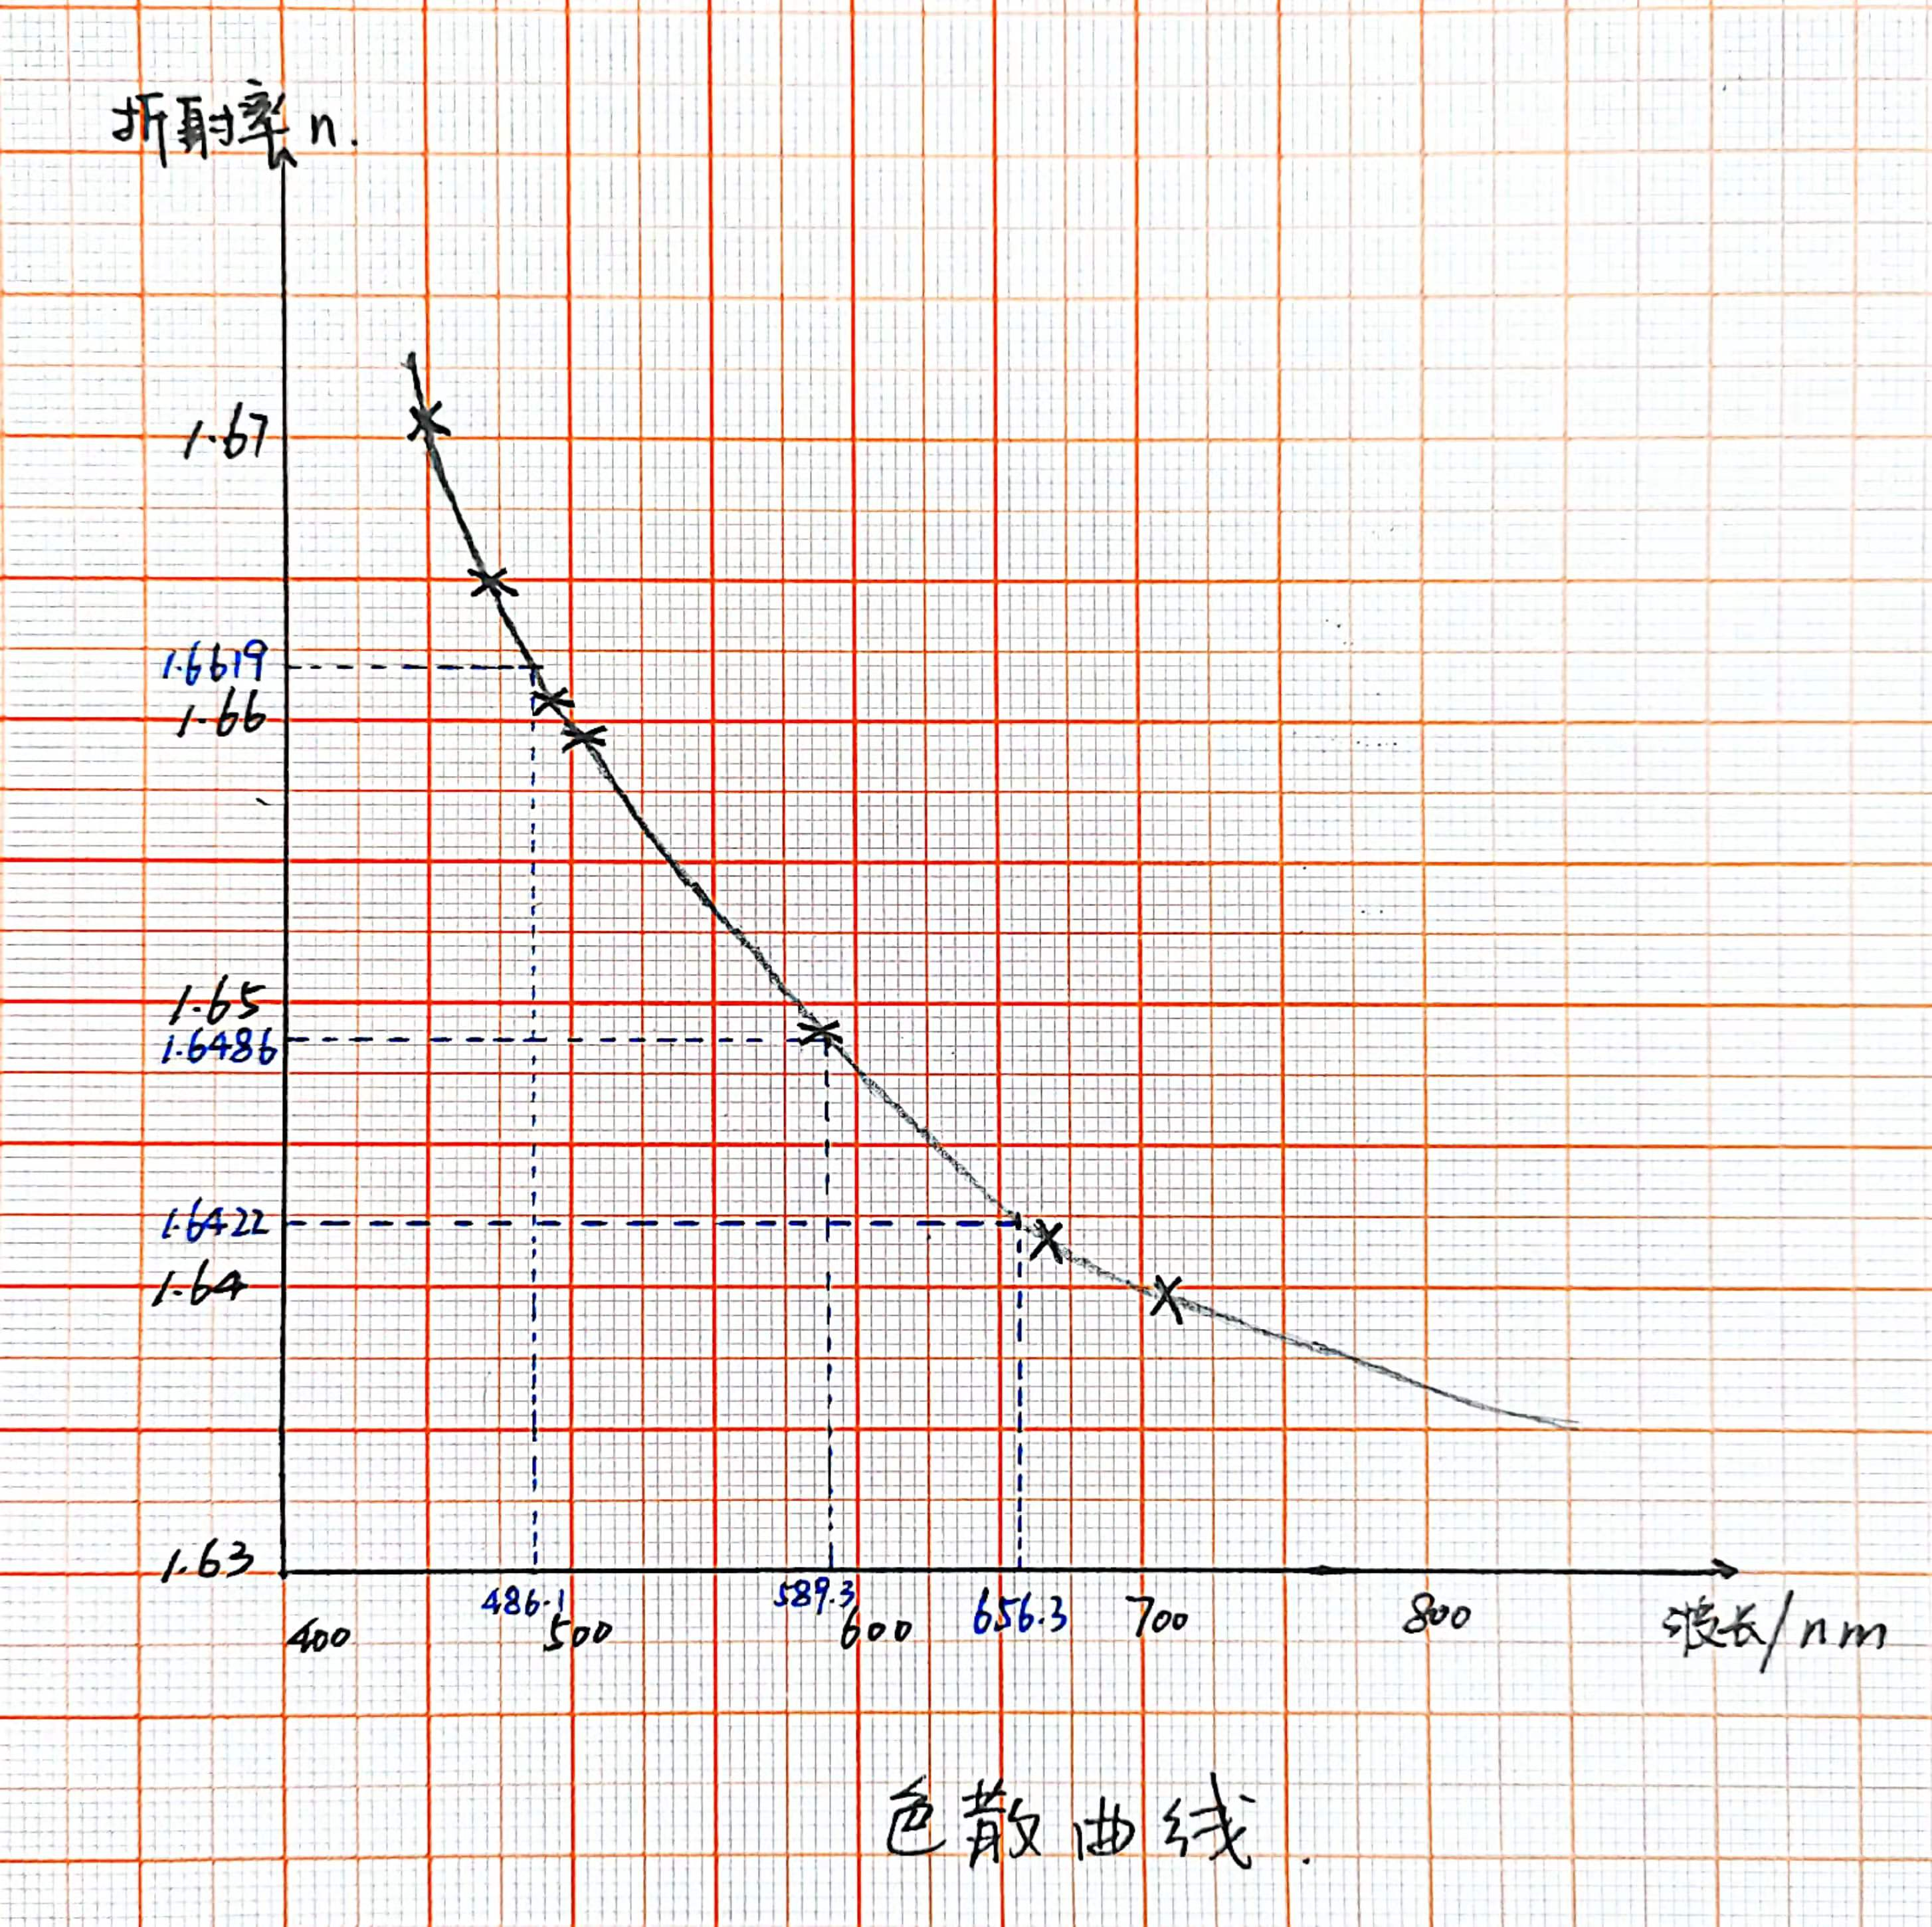
\includegraphics[scale=0.09]{手绘色散曲线.jpg}
\end{figure}

根据绘图法绘出的色散曲线可以读取出:  $\lambda_{C}=656.3 \mathrm{~nm}$ 、 $\lambda_{D}=589.3 \mathrm{~nm}$ 、 $\lambda_{F}=486.1 \mathrm{~nm} $ 时
折射率  $n_{C}=1.6422$ 、$ n_{D}=1.6486 $、 $n_{F}=1.6619$  。 
计算得平均色散$n_{F}-n_{C}=1.6619-1.6422=0.0197$。

色散本领:
$$
V=\frac{n_{F}-n_{C}}{n_{D}-1}=\frac{0.0197}{1.6486-1}=0.03037
$$

\subsection{多元线性回归求取经验公式}

设折射率 n 与波长 $ \lambda  $的关系符合经验公式:
  $$
  n^{2}=A_{0}+A_{1} \lambda^{2}+A_{2} \lambda^{-2}+A_{3} \lambda^{-4}+A_{4} \lambda^{-6}+A_{5} \lambda^{-8}
  $$  

利用计算机进行回归分析后所得的拟合公式系数如下表所示:\\

\begin{tabular}{|c|c|c|c|c|c|}
    \hline $A_{0}$ & $A_{1} $& $A_{2}$ & $A_{3}$ & $A_{4}$ & $A_{5}$ \\
    \hline 1.0246 & $1.0323 \times 10^{-6}$ & $9.8479 \times 10^{5}$ & $-2.7310 \times 10^{11}$ & $3.7807 \times 10^{16}$ &$ -2.0225 \times 10^{21}$ \\
    \hline
\end{tabular}\\


使用matlab绘图如下:

\begin{figure}[H]
    \centering
    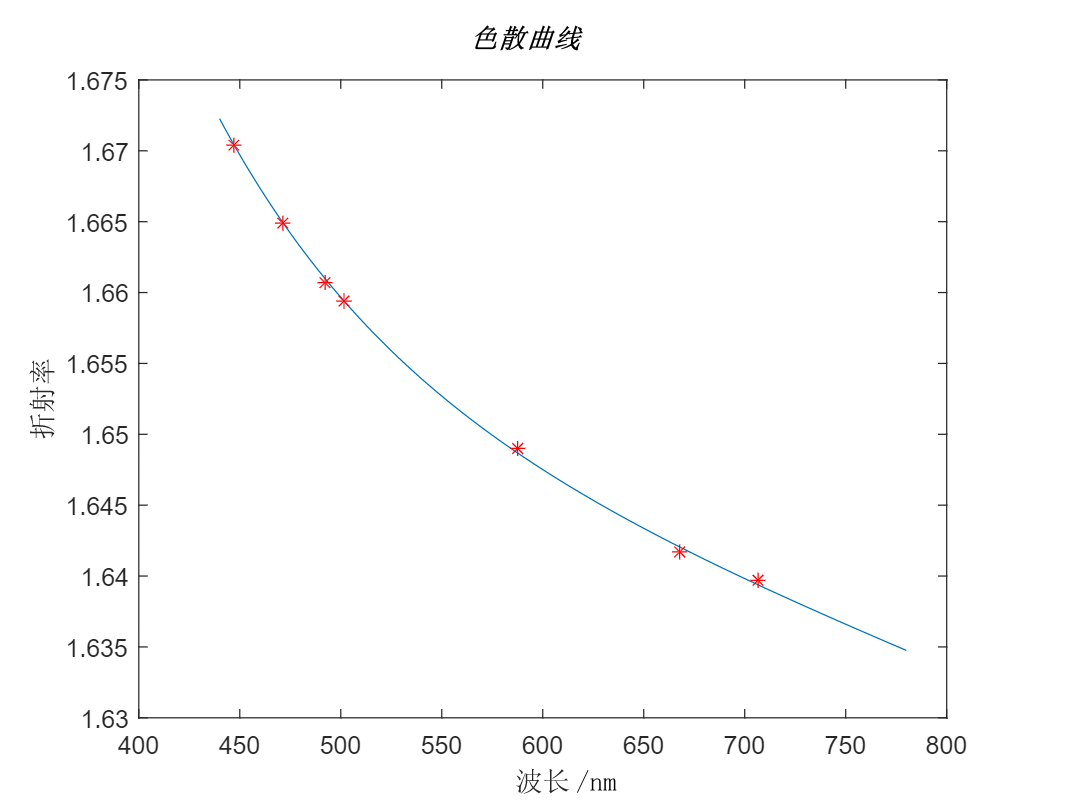
\includegraphics[scale=0.8]{色散曲线.png}
\end{figure}

可计算出:  $\lambda_{C}=656.3 \mathrm{~nm}$ 、 $\lambda_{D}=589.3 \mathrm{~nm}$ 、 $\lambda_{F}=486.1 \mathrm{~nm} $ 时
折射率  $n_{C}=1.6425$ 、$ n_{D}=1.6486 $、 $n_{F}=1.6618$  。 
计算得平均色散$n_{F}-n_{C}=1.6618-1.6425=0.0193$。

色散本领:
$$
V=\frac{n_{F}-n_{C}}{n_{D}-1}=\frac{0.0193}{1.6486-1}=0.02975
$$

以作图法为参考,拟合曲线算出的平均色散和色散本领的相对偏差为2.03\%和2.04\%,
说明经验公式可以较准确地描述色散特性。

\section{实验总结}

\noindent \textbf{思考题}

\noindent  \textbf{(1) 当转动小平台 180°反复调节使望远镜光轴垂直于分光计主轴时,小平台是否也同时调好到垂直于主
轴了?为什么?}

小平台不一定调好到垂直于主轴,原因有二:

1.平面镜与小平台接触面不一定与平面镜法线平行,故即使法线垂直于主轴,接触面也不一定垂直于主轴,即平台不一定垂直于主轴;

2.平面镜法线垂直于主轴后,当平台绕平面镜法线发生偏转时,并不影响平面镜法线与主轴垂直关系,故即使接触面平整,
平台也可能与主轴不垂直。


\noindent  \textbf{(2)根据折射定律,请结合下图定性分析入射光的方位应处于何种情况时才可能找到最小偏向角?}

\begin{figure}[H]
    \centering
    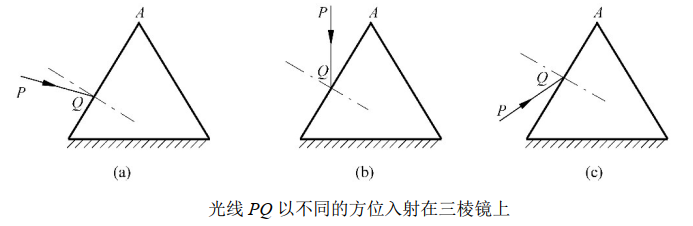
\includegraphics[scale=0.9]{思考题.png}
\end{figure}

图(c)最可能找到最小偏向角,定性绘制光路图如下:

\begin{figure}[H]
    \centering
    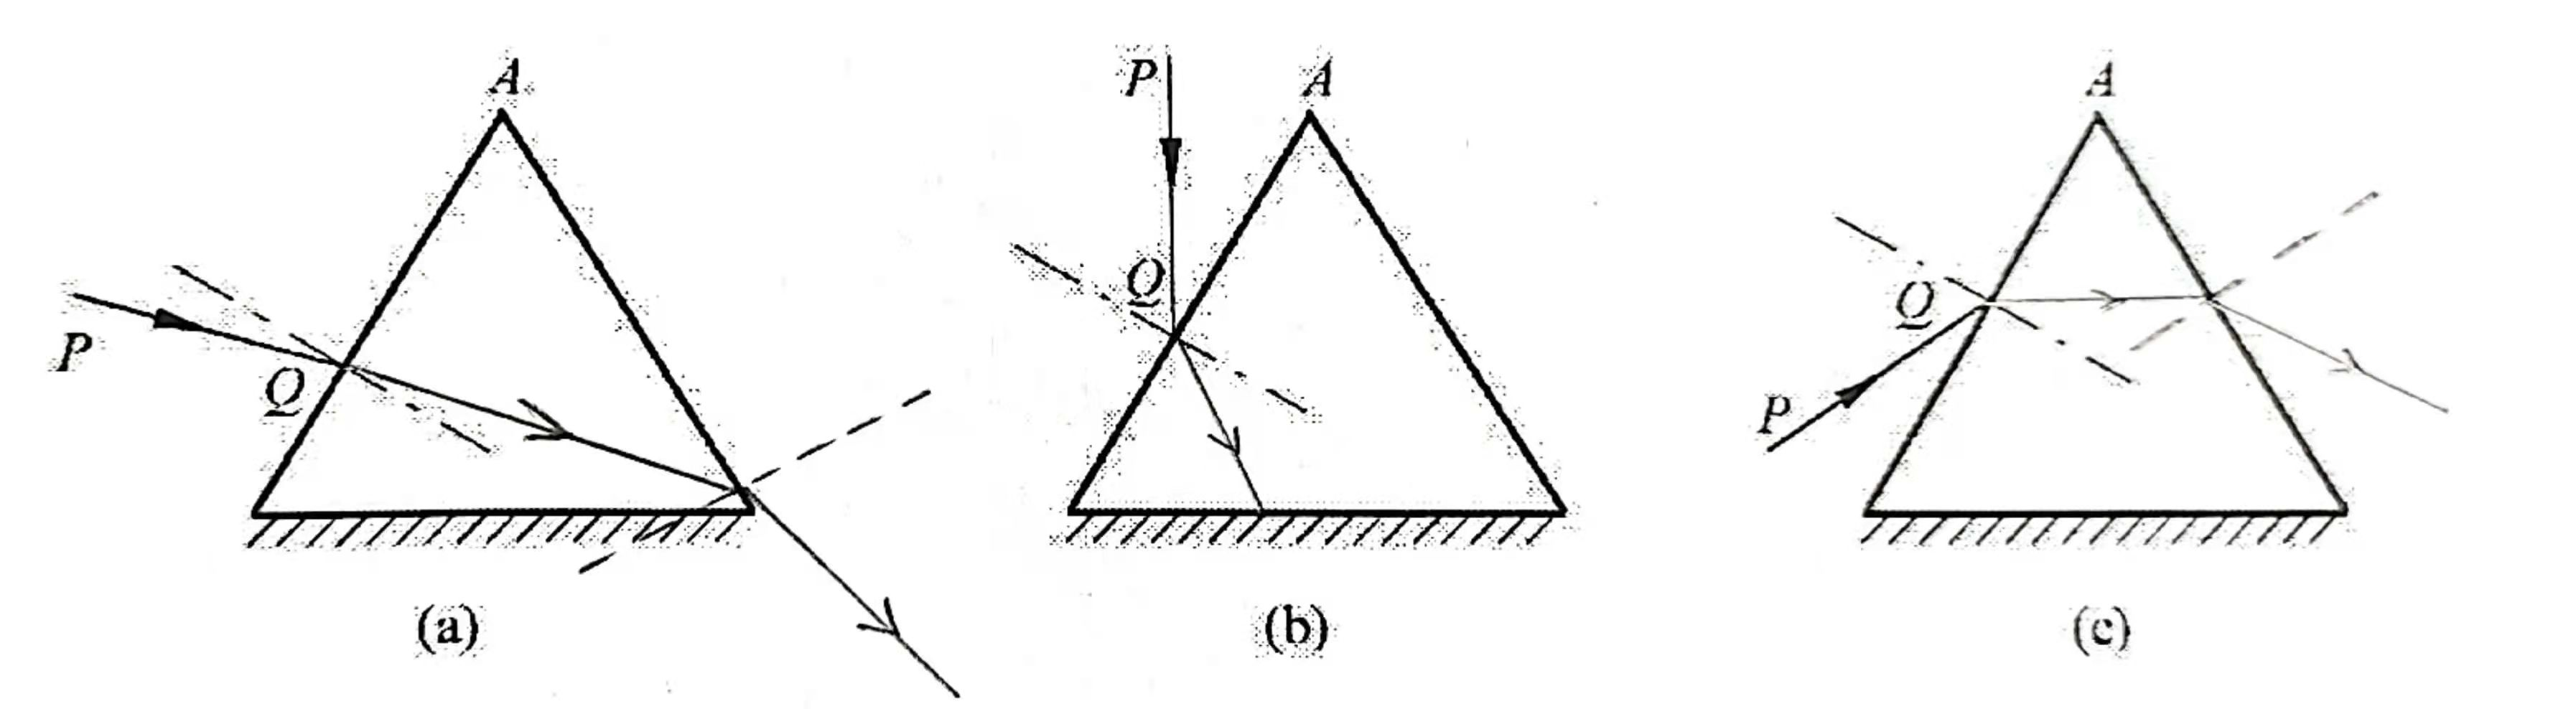
\includegraphics[scale=0.09]{手绘光路.jpg}
\end{figure}

根据折射定律, 折射光与入射光分居法线两侧,出射角过大时会发生全反射。 

图(b)中, 入射点 Q 靠近非光学面, 则在调整和观察过程中折射光线很可能射向非光学面,
而且出射角较大可能发生全反射,所以不容易观测到清晰的谱线; 

图(a)入射光线在法线的右侧,大概率射向非光学面,而非光学面的反射光线较弱不易被观测,故也不容易观测到清晰地谱线。

综上图c最可能找到最小偏向角。

\noindent  \textbf{(3)根据本实验的原理怎样测量光波波长?}

1.用分光计测出三棱镜对该光的最小偏向角$\delta$;

2.利用自准法测量三棱镜顶角 A;

3.利用公式 $n=\sin \frac{A+\delta}{2} / \sin \frac{A}{2}$计算折射率 $n_0$;

4.利用绘制出的色散曲线,在曲线上找到纵坐标为 n 的点,该点横坐标即为光波长的测量值。

~~~另外,也可以将 n 代入经验公式,解出 $\lambda$ 即为的光波长的测量值。


\noindent  \textbf{(4)试根据光路图分析,为什么望远镜光轴与平面镜法线平行时,在目镜内应看到“+”形反射像与
叉丝的上方交点相重合?}

\begin{figure}[H]
    \centering
    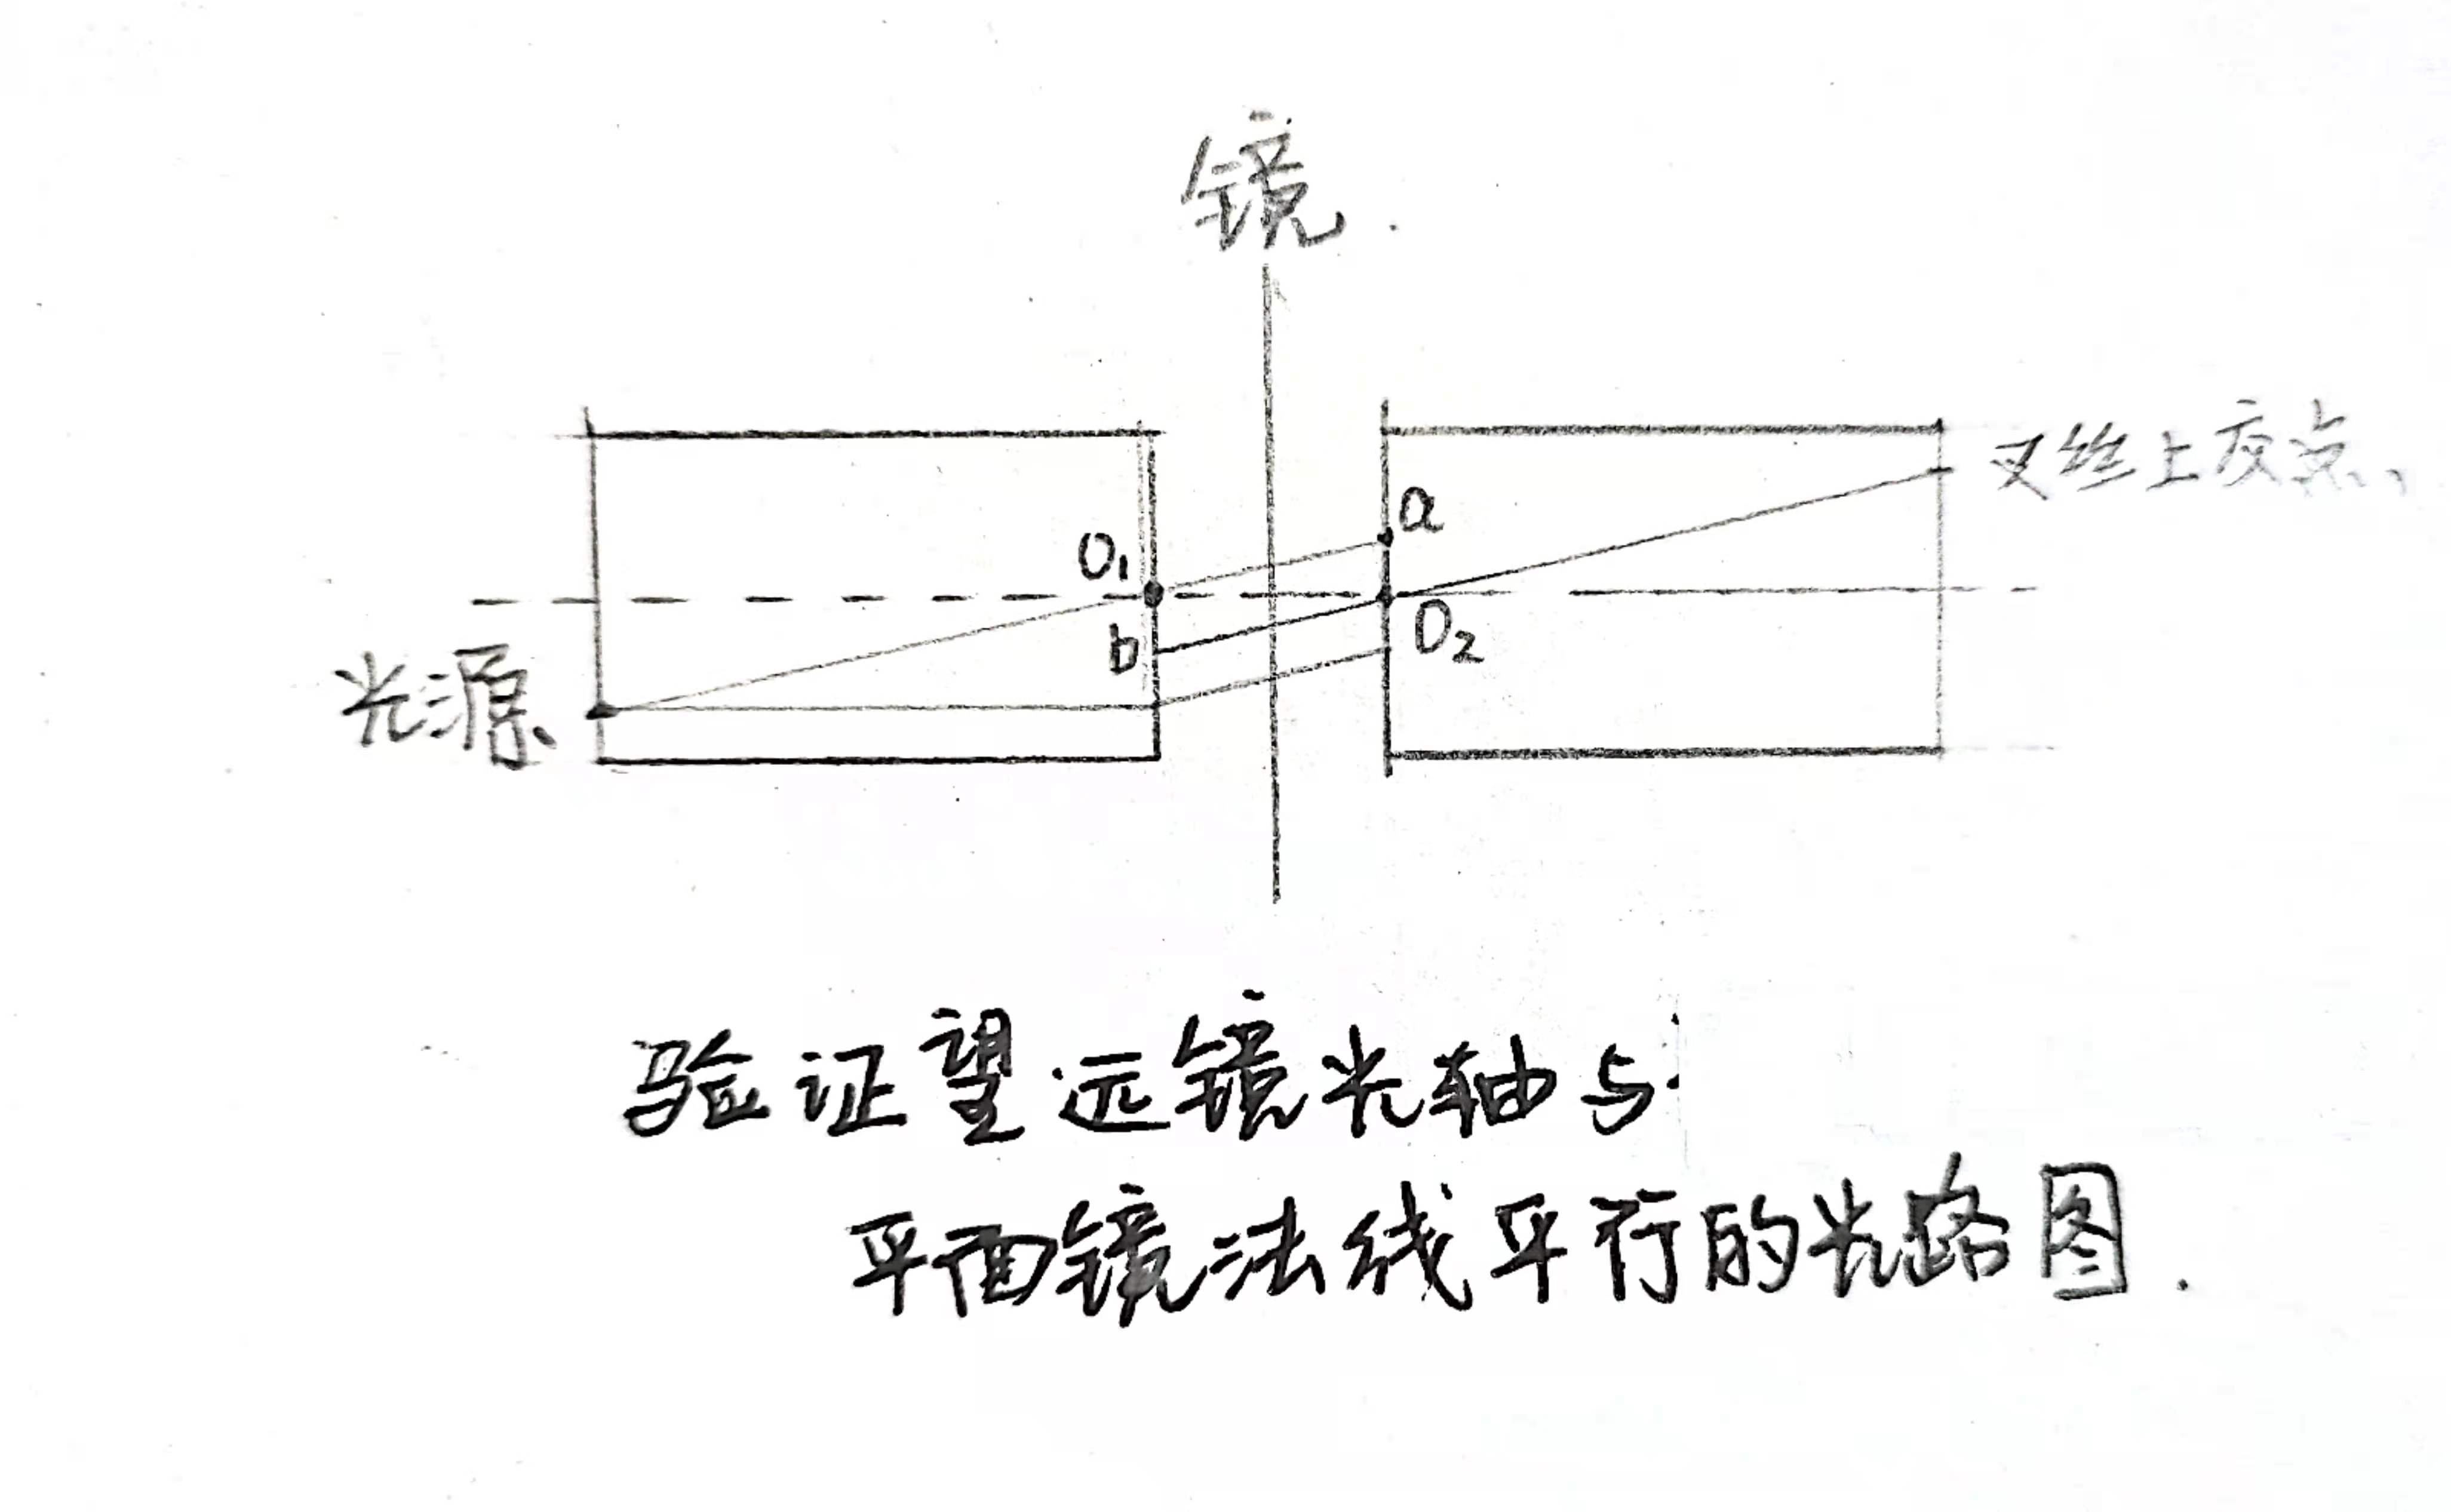
\includegraphics[scale=0.06]{思考题光路.jpg}
\end{figure}

当望远镜光轴与平面镜法线平行时,光路图如上。
由于平面镜镜面反射的对称性,我们我们可以将光源和叉丝对称绘制来观察光路。
可以预见,光源一定会发出过透镜中心的$O_1a$光线,那么由于光源在焦平面上,
出射光线都平行,所以一定有光线$bO_2$而且与$O_1a$平行,而$bO_2$过$O_2$,
所以与焦平面交于与光源对称的叉丝上交点,而平行光经过凸透镜必定汇聚于焦平面上一点,
那么十字形反射像就会汇聚在焦平面上与叉丝上交点重合处。\\

\noindent  \textbf{总结:}

经过这次实验我学会了分光计的调节和使用方法,自准法测三棱镜顶角的操作方法,
用最小偏转角测量折射率的原理和操作方法。

此外我还了解到了一些实验注意事项以及操作技巧,例如:
拿取光学元件时只能接触磨砂面,要轻拿轻放,切勿用手接触光学表面;分光计螺钉的拧动原则;
为消除偏心差,需要采用两个相差180度的窗口读数。

在实验中我遇到了一些问题:比如在调整好仪器之后观测不到谱线,
经过老师指导后我了解到,一方面我观察到的断断续续的光谱是其他光源传播过来的,
另一方面观察不到我的光源产生的光谱是因为三棱镜的摆放位置和角度不合适导致
出射光线射向了非光学面或者发生了全反射。最后经过调整成功观测到了谱线
、测量了全部7条谱线的数据并通过验收。

最后感谢老师的悉心指导!

(原始实验记录见下页)

\section{原始数据记录}

\begin{figure}[H]
    \centering
    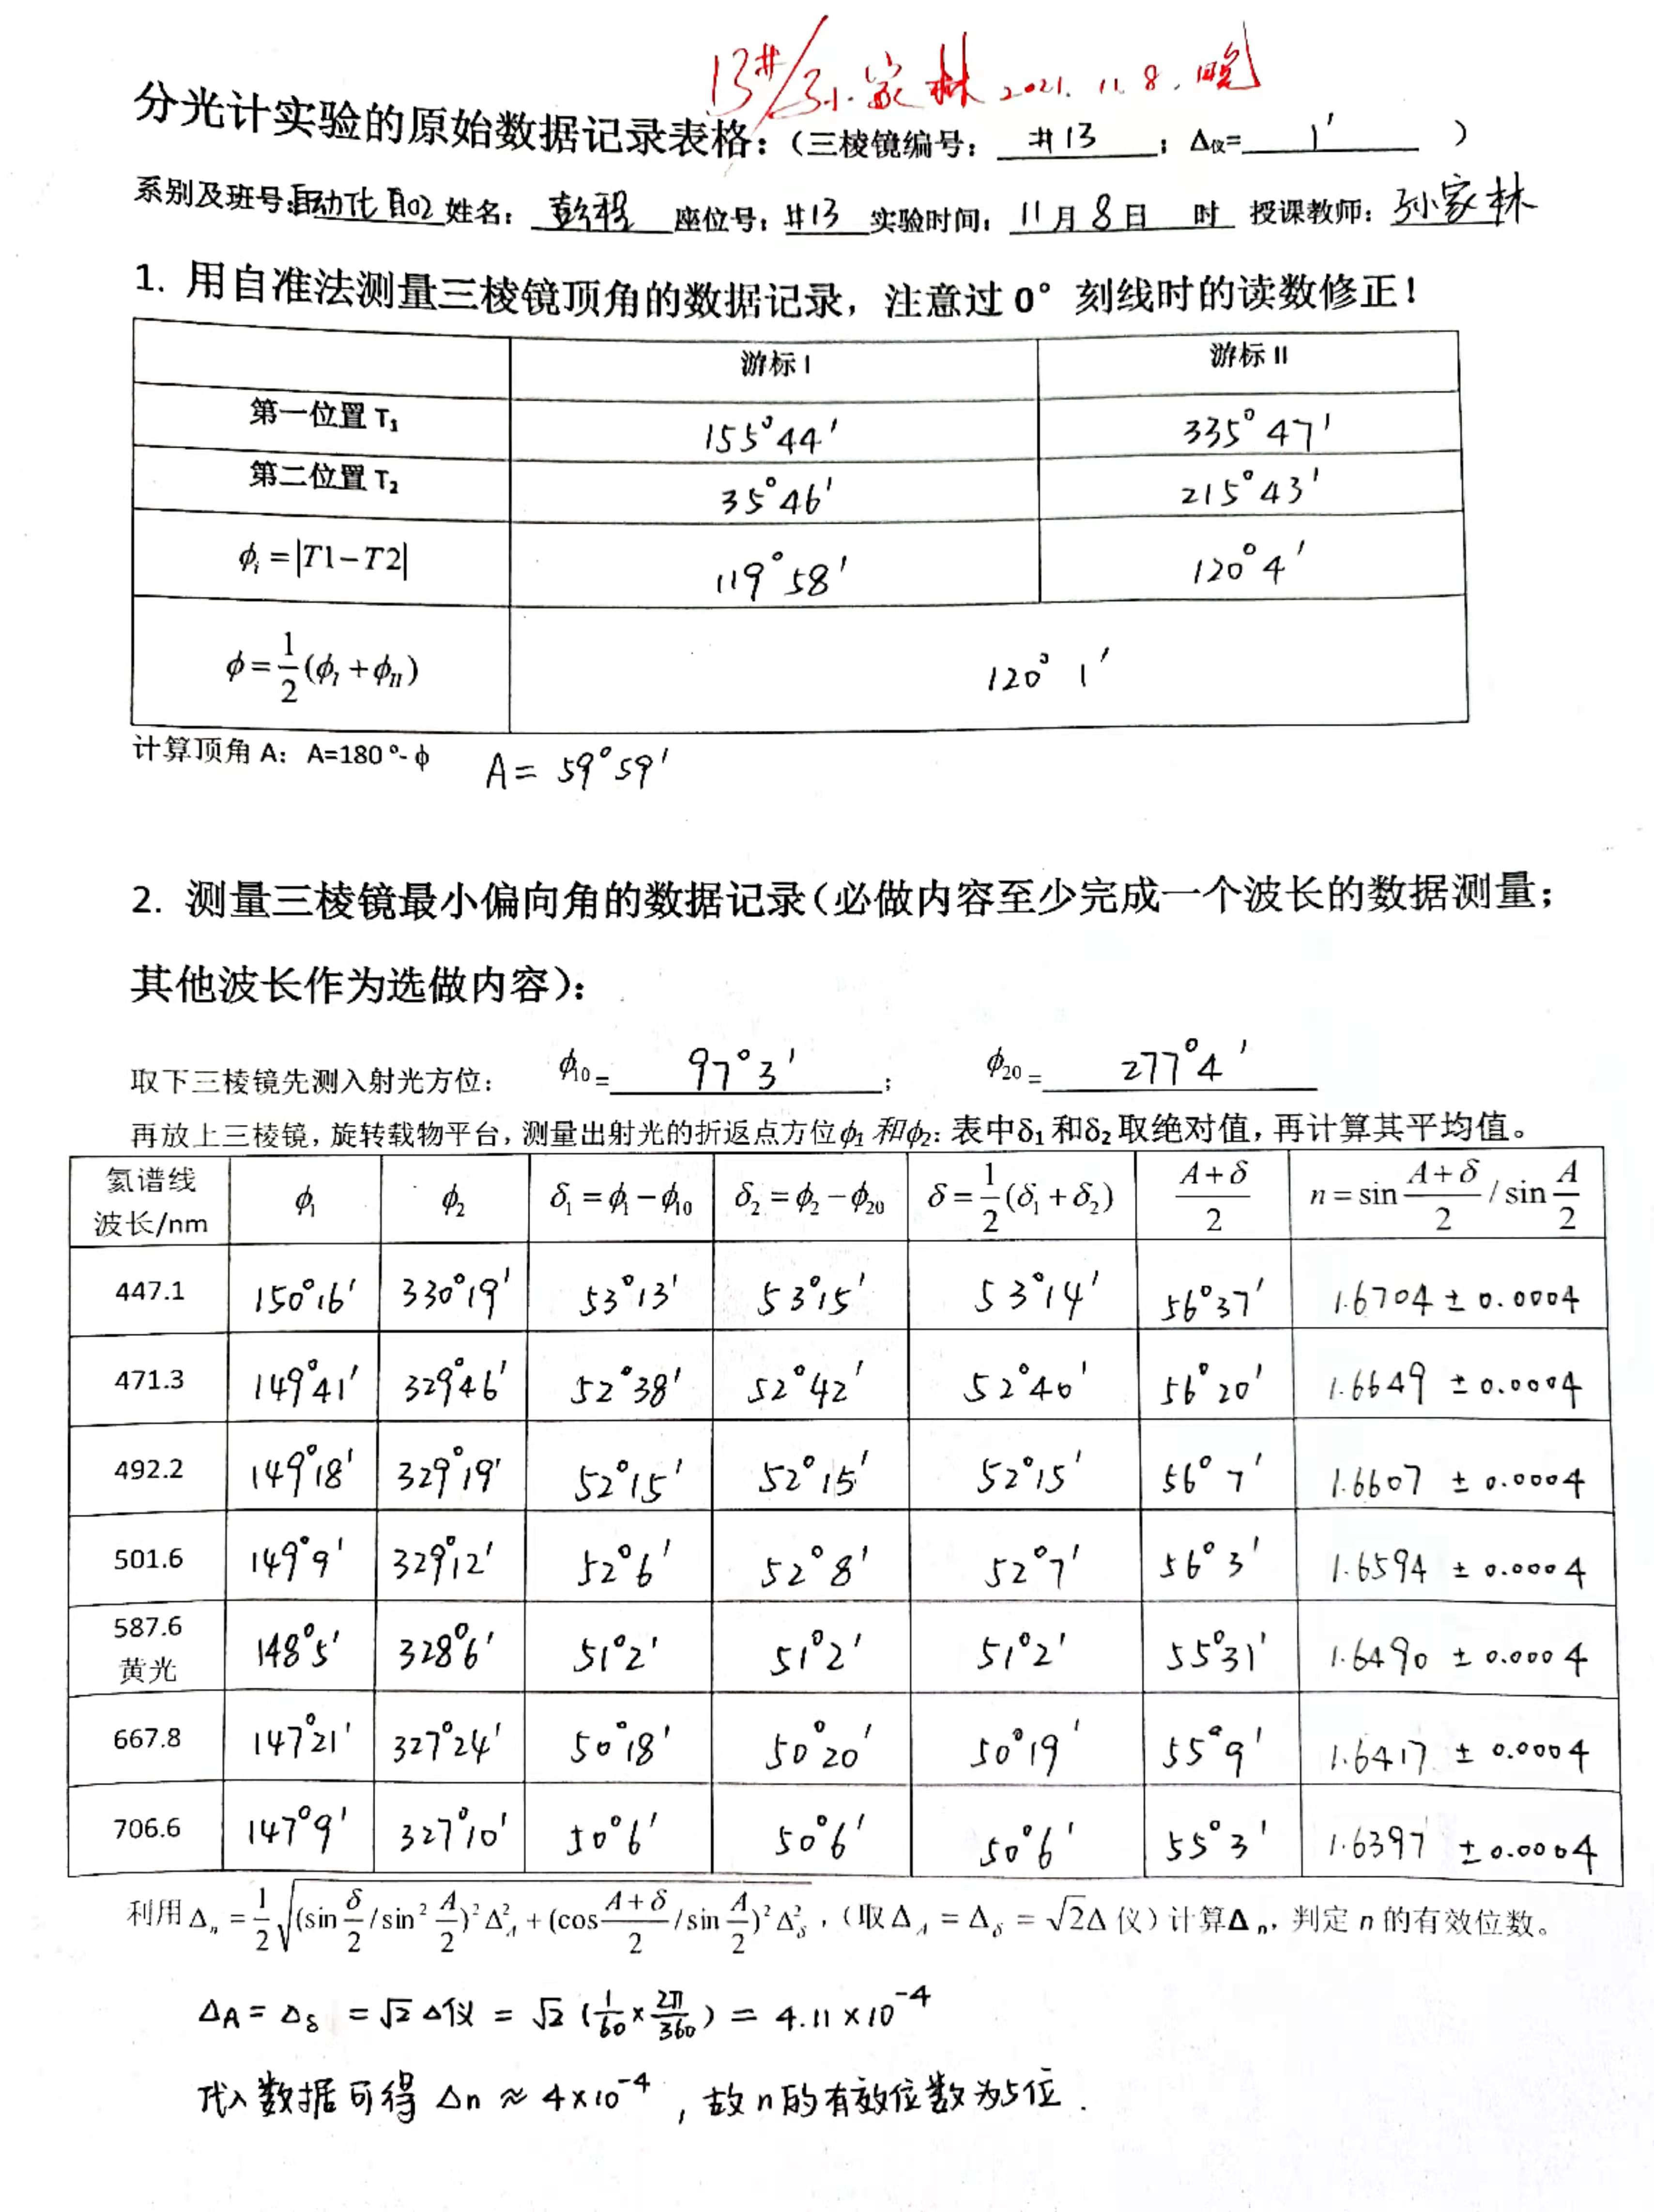
\includegraphics[scale=0.13]{分光计原始数据.jpg}
    
\end{figure}

\end{document}